% ============================================================
% 2B
% ============================================================

\section{Task 2B: SIMD (Single Instruction Multiple Data)}

\subsection{SIMD Implementation}
To parallelize the SGEMM operation, we implemented a register-blocked SIMD micro-kernel using AVX2 intrinsics. We unrolled the outer loops to compute a $2 \times 4$ block of the output matrix $C$ simultaneously. For the inner dot-product loop across the $K$ dimension, we used \texttt{\_mm256\_loadu\_ps} to fetch 8 elements from both matrices and accumulated the results using \texttt{\_mm256\_fmadd\_ps}. Finally, we implemented a \texttt{horizontal\_sum} helper function using vector extraction and addition to collapse the 8-lane accumulators into scalar values for the final output. 

\subsection{Performance and Instruction Analysis}

As expected, vectorizing the dot product drastically reduced the number of executed instructions. For a $1024 \times 1024$ matrix, the baseline executed $\sim$6.46 billion instructions, whereas the 256-bit SIMD implementation required only $\sim$227 million instructions—a reduction by a factor of roughly $28\times$.

\begin{table}[H]
\centering
\caption{Task 2B Execution Time and Speedup Summary}
\begin{tabular}{lccc}
\toprule
Matrix Size & No SIMD Time (ms) & 128-bit Speedup & 256-bit Speedup \\
\midrule
$128 \times 128$ & 0.76 & 8.67$\times$ & 12.64$\times$ \\
$256 \times 256$ & 6.20 & 9.11$\times$ & 9.87$\times$ \\
$512 \times 512$ & 53.52 & 9.64$\times$ & 12.15$\times$ \\
$1024 \times 1024$ & 446.38 & 9.19$\times$ & 11.49$\times$ \\
$2048 \times 2048$ & 3802.51 & 8.51$\times$ & 10.00$\times$ \\
\bottomrule
\end{tabular}
\end{table}

\begin{figure}[H]
    \centering
    \begin{subfigure}{0.48\textwidth}
        \centering
        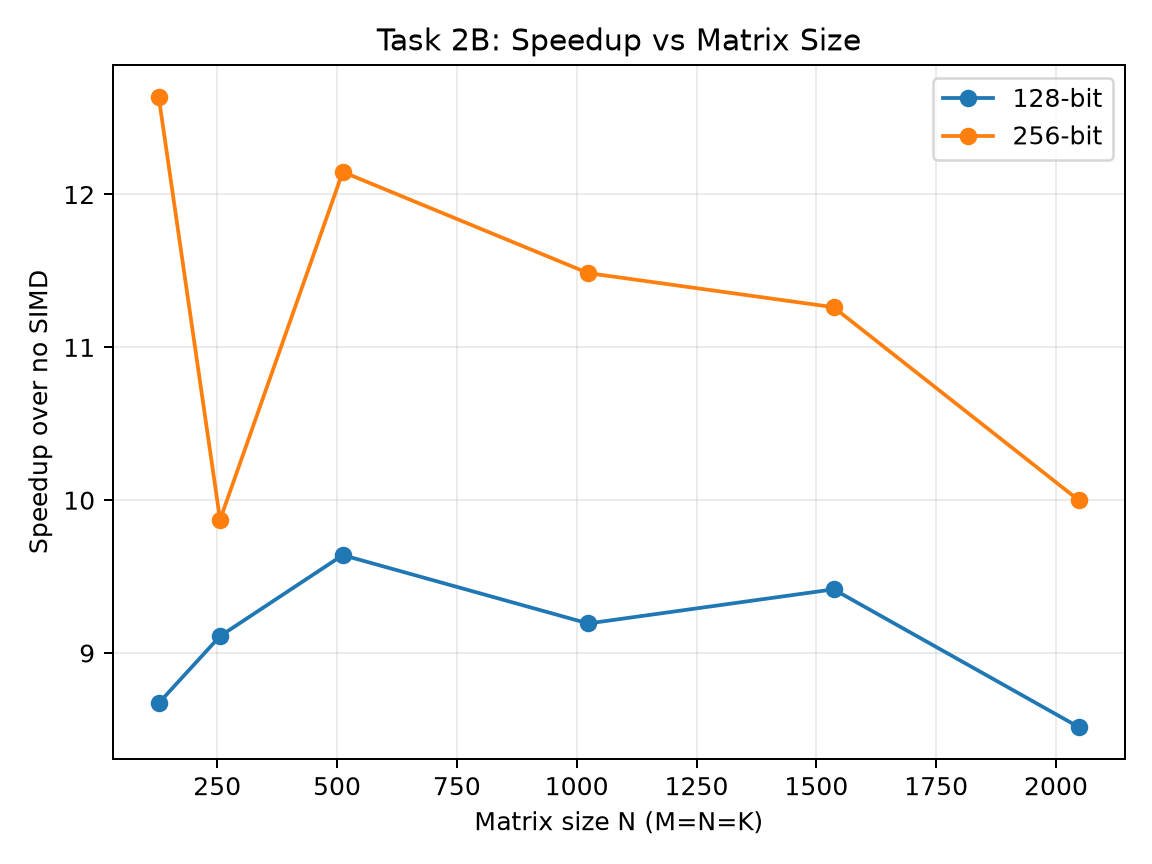
\includegraphics[width=\linewidth]{plots/task2b/task2b_speedup_vs_size.png}
        \caption{Speedup vs Matrix Size}
    \end{subfigure}
    \hfill
    \begin{subfigure}{0.48\textwidth}
        \centering
        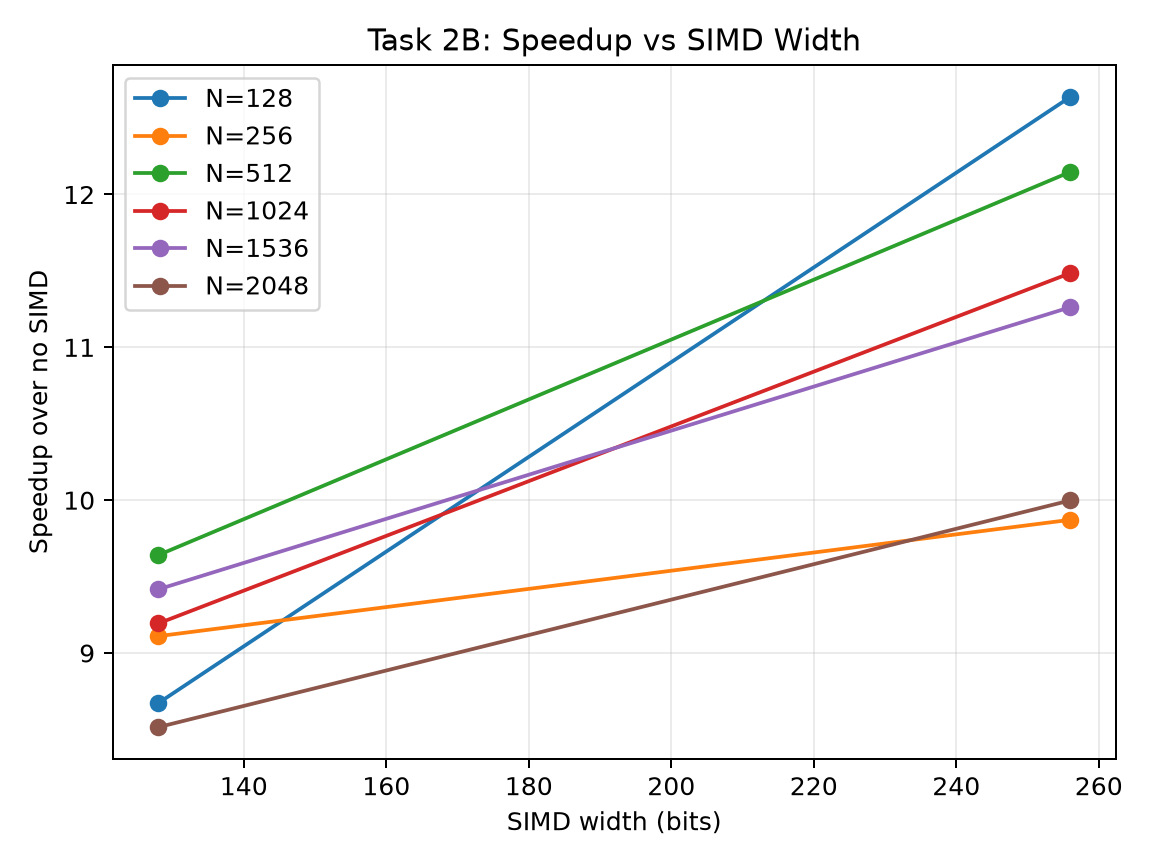
\includegraphics[width=\linewidth]{plots/task2b/task2b_speedup_vs_width.png}
        \caption{Speedup vs SIMD Width}
    \end{subfigure}
    \caption{Performance improvements across varying matrix constraints.}
\end{figure}

\begin{figure}[H]
    \centering
    \begin{subfigure}{0.48\textwidth}
        \centering
        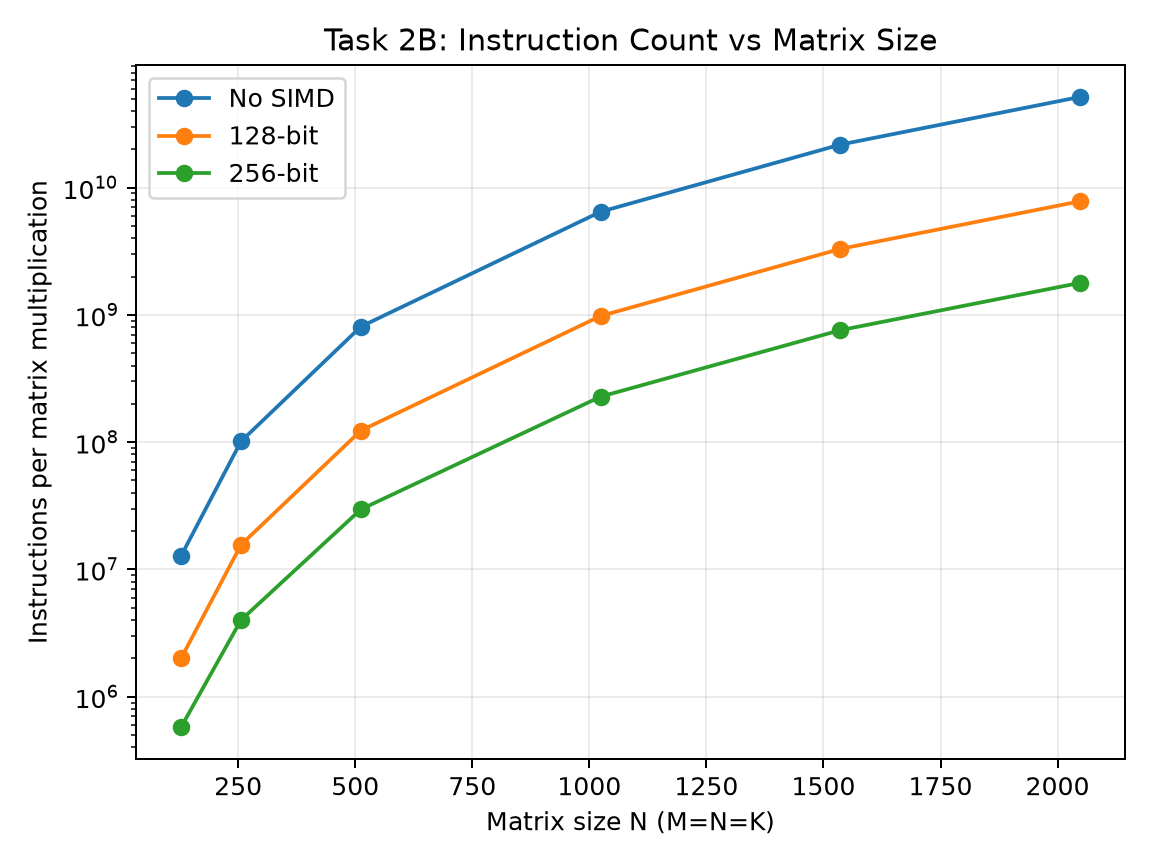
\includegraphics[width=\linewidth]{plots/task2b/task2b_instructions_vs_size.png}
        \caption{Total Instructions vs Size}
    \end{subfigure}
    \hfill
    \begin{subfigure}{0.48\textwidth}
        \centering
        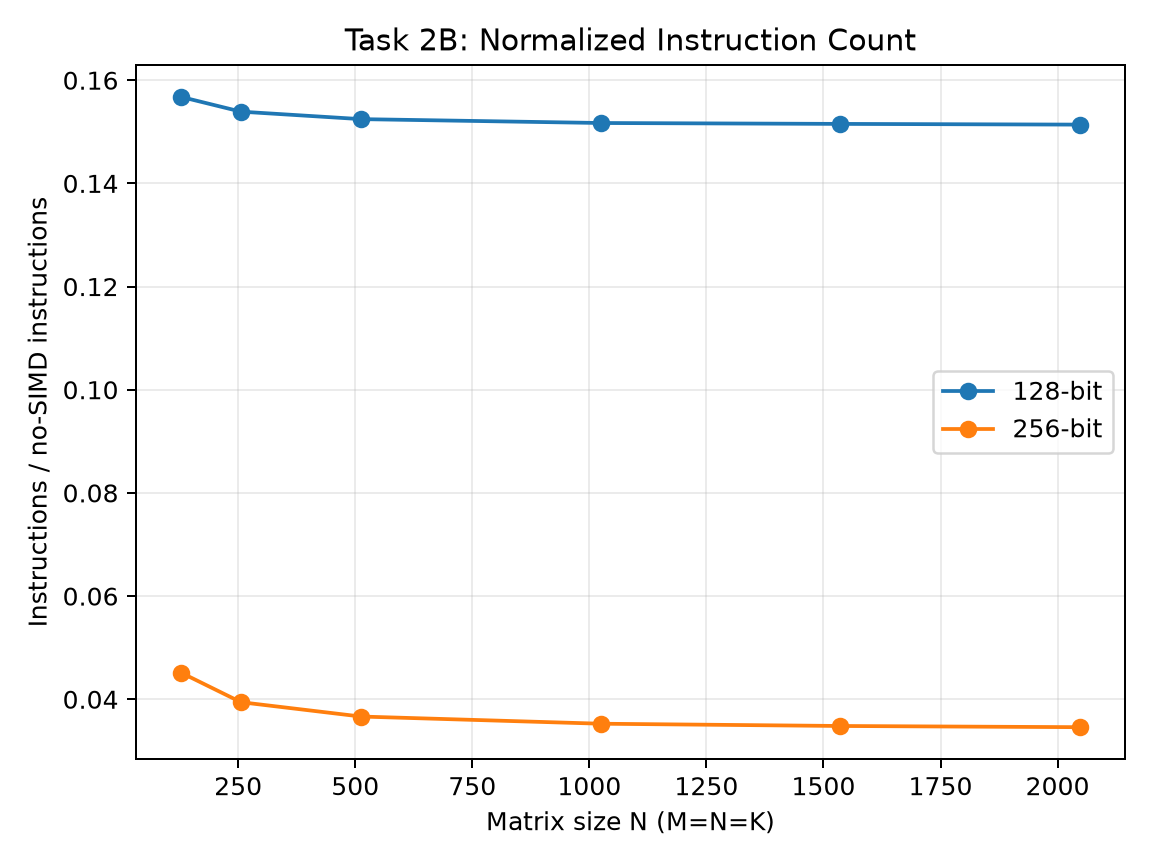
\includegraphics[width=\linewidth]{plots/task2b/task2b_instruction_ratio_vs_size.png}
        \caption{Normalized Instruction Count}
    \end{subfigure}
    \caption{Impact of vectorization on total instruction execution.}
\end{figure}

\begin{figure}[H]
    \centering
    \begin{subfigure}{0.48\textwidth}
        \centering
        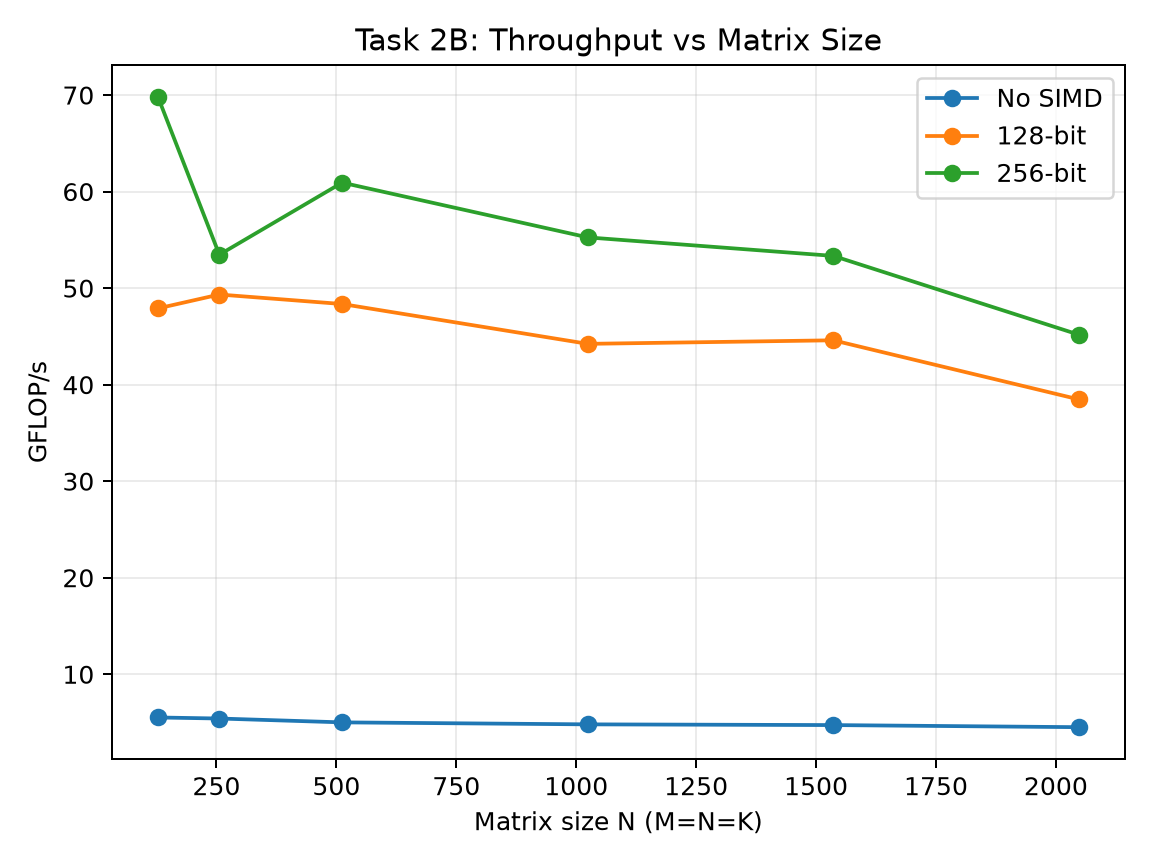
\includegraphics[width=\linewidth]{plots/task2b/task2b_gflops_vs_size.png}
        \caption{Throughput (GFLOP/s) vs Size}
    \end{subfigure}
    \hfill
    \begin{subfigure}{0.48\textwidth}
        \centering
        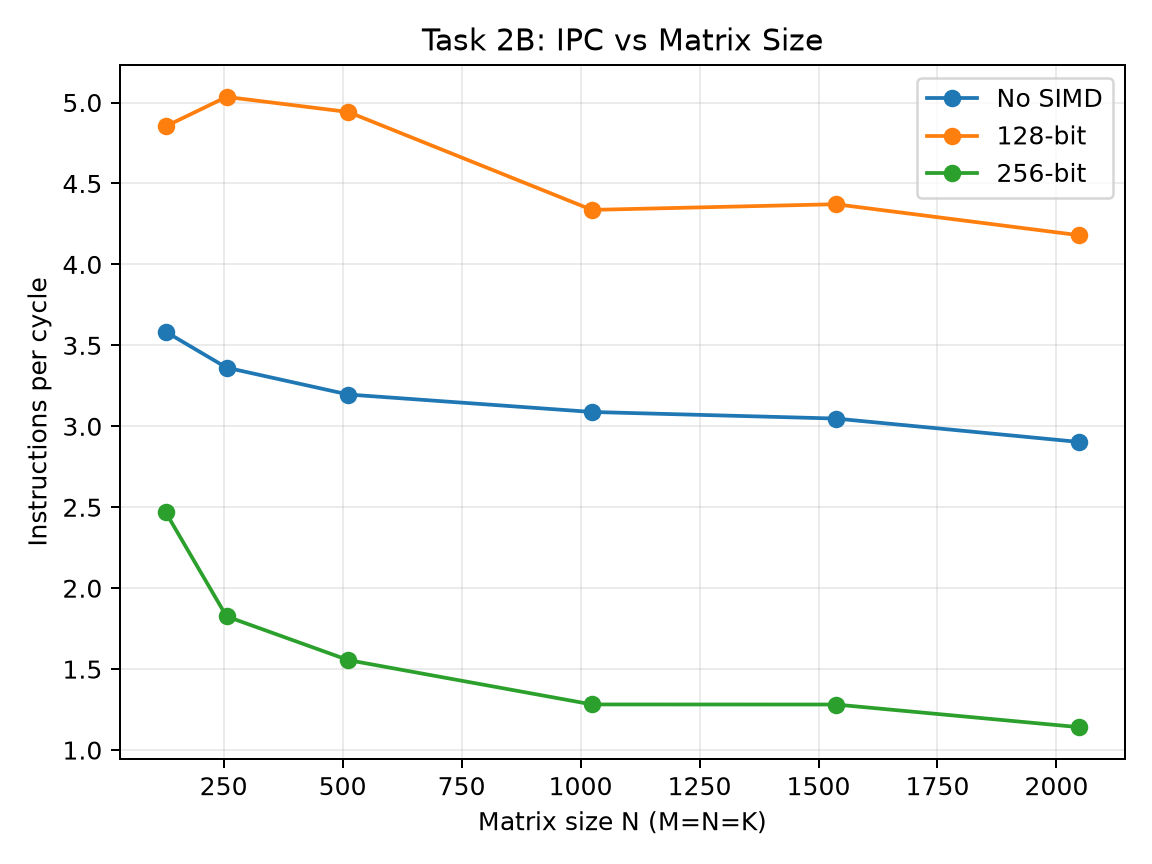
\includegraphics[width=\linewidth]{plots/task2b/task2b_ipc_vs_size.png}
        \caption{IPC vs Size}
    \end{subfigure}
    \caption{Hardware utilization and throughput efficiency.}
\end{figure}


\subsection{Questions}

\begin{enumerate}
    \item \textbf{What trends do you observe in speedup for different combinations of matrix sizes and SIMD widths?} \\
    The 256-bit SIMD implementation strictly outperforms the 128-bit implementation across all matrix sizes. For both widths, the speedup peaks at smaller boundaries (e.g., $12.64\times$ at $N=128$) and gently degrades as the matrix size increases (dropping to $10.00\times$ at $N=2048$). This downward trend indicates that as the matrix footprint grows well beyond the L1/L2 cache capacities, memory bandwidth becomes the primary bottleneck, starving the highly efficient SIMD arithmetic units.
    
    \item \textbf{For which SIMD width do you achieve the maximum speedup?} \\
    We achieved the maximum speedup using the 256-bit SIMD width. It produced a geometric mean speedup of roughly $11.19\times$ across all sizes, compared to the 128-bit version which was consistently slower. This maps directly to the hardware capability: 256-bit registers process 8 single-precision floats per instruction cycle, effectively doubling the raw arithmetic throughput over 128-bit SSE registers.
\end{enumerate}